The data model must be adaptable yet consistent. Users should be able to request collections of linked resources regardless the genre or language of the works involved. Furthermore, they should be able to combine repertories through shared vocabularies and metadata fields. As such, we face an age-old dilemna. We are pulled between being specific and idiosyncratic, on the one hand, and being simple and generalizable on the other. To confront this issue, we first turn to other successful data models. From those precedents, we adopt a hierarchical approach and certain ontological distinctions, notably distinctions between a \textit{Work} (the story), a \textit{Text} (a telling of the story), and a \textit{Witness} (a written version of that telling).

\subsection{Functional Requirements for Bibliographic Records}
One of the most robust bibliographic data models is the Functional Requirements for Bibliographic Records (FRBR), which slowly solidified during the last quarter of the twentieth century and is still today used to structure bibliographic databases.\footcite[][]{FRBR_Worldcat} In 1961, information scientists from around the world gathered in Paris to discuss best practices for cataloguing. Following their Paris meeting, the International Federation of Library Associations (IFLA) supported further discussions and members developed theoretical frameworks for organizing bibliographic data. Finally, in 1997, the IFLA approved the FRBR.\footcite{FRBR_1998} The FRBR articulates a generalizable hierarchy of four related entities: Works (\textbf{W}), Expressions (\textbf{E}), Manifestations (\textbf{M}), and Items (\textbf{I}). One of the examples in the 2009 corrected edition demonstrates how these entities relate to one another through the case of Johann Sebastian Bach's Goldberg variations.\footcite[We have augmented the example by adding an Item.][58]{FRBR_2009}

\begin{itemize}
    \item \textbf{W\textsubscript{1}} J. S. Bach's Goldberg variations
    \begin{itemize}
        \item \textbf{E\textsubscript{1}} performances by Glenn Gould recorded in 1981
        \begin{itemize}
            \item \textbf{M\textsubscript{1}} recording released on 33 1/3 rpm sound disc in 1982 by CBS Records
            \item \textbf{M\textsubscript{2}} recording re-released on compact disc in 1993 by Sony
            \begin{itemize}
                \item \textbf{I\textsubscript{1}} copy held at Cook Music Library, Bloomington, Indiana, USA (WOODWARD CD .B118 K1.988-35)
            \end{itemize}
        \end{itemize}
    \end{itemize}
\end{itemize}

In the FRBR model, a \textit{Work} is ``a distinct intellectual artistic creation'' and can have a title, a date, and a form or genre.\footcite[][17]{FRBR_2009} An \textit{Expression} is an ``intellectual or artistic realization'' of the \textit{Work} in some specific form, such as alpha-numeric or musical notation, sound, image, or movement.\footcite[][19]{FRBR_2009} Manifestations are the concrete, ``physical embodiment'' of the \textit{Expression} of a \textit{Work}.\footcite[][21]{FRBR_2009} For instance, if an \textit{Expression} of a \textit{Work} is notated in Vedic Sanskrit around 900 BCE, a \textit{Manifestation} of that literary \textit{Expression} would be a physical manuscript. Finally, an Item is a ``single exemplar of a manifestation,'' which is a concept best suited for mass-produced resources, such as copies of an edited book or, as in the example above, copies of a CD-ROM.\footcite[][24]{FRBR_2009}

% \begin{table}[ht]
% \begin{center}
    \begin{tabular}
        {|p{0.06\textwidth}|p{0.15\textwidth}|p{0.7\textwidth}|}
        \hline
        \textbf{Depth} & \textbf{FRBR Entity} & \textbf{Test Case} \\
        \hline
        1 & Work & One story of Renaut de Montauban and his brothers (\textit{The four sons of Aymon}).\\
        \hline
        2 & Expression & David Aubert’s prosified version of the story, known as \textit{Renaut de Montauban}.\\
        \hline
        3 & Manifestation & A copy of Aubert’s version, which was composed in five volumes in the 1460s.\\
        \hline
        4 & Document & One of the copy's volumes, i.e. Bibliothèque nationale de France, Arsenal, français, MS 5072.\\
        \hline
    \end{tabular}
\end{center}
% \caption{FRBR with test case \textit{Renaut de Montauban}.}
% \end{table}

% \subsection{\textit{Encoded Archival Standards}}
% The Encoded Archival Standards (EAD) is an international set of bibliographic protocols whose first definitive version, 1.0, was recently released in 2024. When encoded in EAD, the item's electronic record has two main components: information about the record itself (\texttt{<control>}), and information about the archival item (\texttt{<archdesc>}). The latter is relevant to the resources in LostMa's data model and includes the following sections:

\begin{itemize}
    \item Descriptive Identifier (\texttt{<did>}) : identifies the constitution of the archival item and other identifying information
    \begin{itemize}
        \item Title
        \item Author
        \item Date
        \item Repository
        \item Language
    \end{itemize}
    \item Scope Content (\texttt{<scopecontent>}) : meaningfully describes the content in the archival item
\end{itemize}

\subsection{\textit{Textrad}}
More recently this century, Patrick Sahle has developed a set of entity relationships that have significantly impacted the fields of philology and textual criticism.\footcite{Sahle2013} At the core of his wheel model (\textit{Textrad}), which we illustrate as a triangle in Figure \ref{fig:Textrad}, Sahle deconstructs the idea of a text into three primary dimensions: text as a story's ideal content \brackettext{\textit{Inhalt}}, not mediated by anything (\textbf{I}); text as a story's linguistic content \brackettext{\textit{sprachlichem Gehalt}}, mediated through human language (\textbf{S}); and text as a physical document \brackettext{\textit{Dokument}} (\textbf{D}) on which a story's content is materially represented.

\begin{figure}[ht]
\begin{center}
    \tikzstyle{s} = [rectangle, rounded corners, minimum width=3cm, minimum height=1cm,text centered, draw=black]
    \tikzstyle{arrow} = [thick,->,>=stealth]
    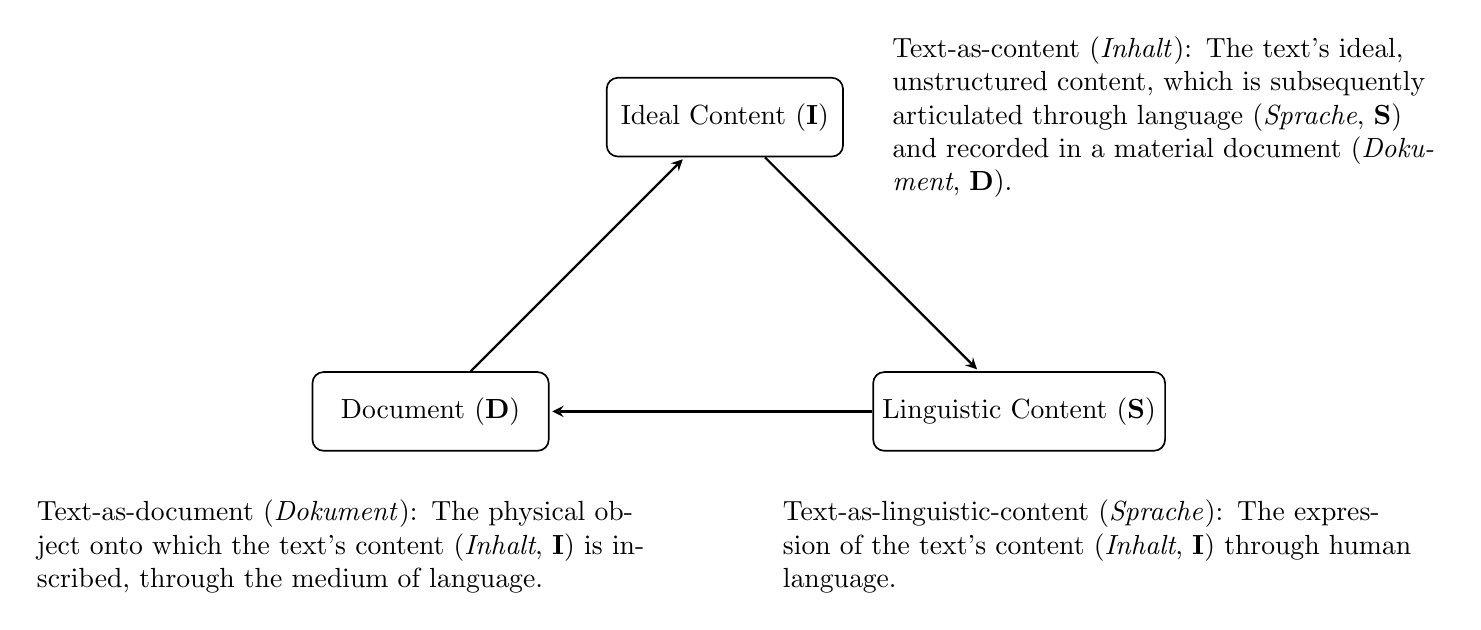
\begin{tikzpicture}[-,shorten >=1pt,auto,node distance=2.8cm,semithick]
    \tikzstyle{every state}=[fill=red,draw=none,text=white]
    \node[s] (D) {Document (\textbf{D})};
    \node[s] (I) [above right of=D, xshift=5em, yshift=5em] {Ideal Content (\textbf{I})};
    \node[s] (S) [below right of=I, xshift=5em, yshift=-5em] {Linguistic Content (\textbf{S})};
    \node [below=1cm,text width=8cm, xshift=1cm] at (S)
    {
    Text-as-linguistic-content (\textit{Sprache}): The expression of the text's content (\textit{Inhalt}, \textbf{I}) through human language.
    };
    \node [below=1cm,text width=8cm, xshift=-1cm] at (D)
    {
    Text-as-document (\textit{Dokument}): The physical object onto which the text's content (\textit{Inhalt}, \textbf{I}) is inscribed, through the medium of language.
    };
    \node [right=2cm,text width=7cm] at (I)
    {
    Text-as-content (\textit{Inhalt}): The text's ideal, unstructured content, which is subsequently articulated through language (\textit{Sprache}, \textbf{S}) and recorded in a material document (\textit{Dokument}, \textbf{D}).
    };
    \draw [arrow] (S) -> (D);
    \draw [arrow] (D) -> (I);
    \draw [arrow] (I) -> (S);
    \end{tikzpicture}
\end{center}
\caption{Main spokes of Sahle's \textit{Textrad}}
\label{fig:Textrad}
\end{figure}

Between the main spokes of the text-wheel (\textit{Textrad}), as seen in Figure \ref{fig:TextradAll}, Sahle includes three other dimensions: text as a set of signs (\textit{Zeichen}), text as a structured sequence of content (\textit{Werk}), and text as a version (\textit{Fassung}). Sahle's embedded dimensions make certain assertions about texts. For example, changes in a text's linguistic content (\textbf{S}), such as translating \textit{Beowulf} from Old English to contemporary Italian, will produce a new version (\textbf{F}) of the text, which will in turn produce a different physical document (\textbf{D}). However, changing \textit{Beowulf} from Old English to contemporary Italian does not necessarily change the work (\textbf{W}) \textit{Beowulf} itself, which still features the same organizing structure of the content of the \textit{Beowulf} story (\textbf{I}).

\begin{figure}[ht]
\tikzstyle{s} = [rectangle, rounded corners, minimum width=3cm, minimum height=1cm,text centered, draw=black, fill=white]
\tikzstyle{arrow} = [thick,->,>=stealth]
\begin{center}
\begin{tikzpicture}[-,shorten >=1pt,auto,node distance=2.8cm,semithick]
\tikzstyle{every state}=[fill=red,draw=none,text=white]
\node[s] (D) {Document (\textbf{D})};
\node[s] (I) [above right of=D, xshift=5em, yshift=5em] {Ideal Content (\textbf{I})};
\node[s] (S) [below right of=I, xshift=5em, yshift=-5em] {Linguistic Content (\textbf{S})};

\begin{pgfonlayer}{bg}    % select the background layer
    \draw [arrow] (S) -> (D);
    \draw [arrow] (D) -> (I);
    \draw [arrow] (I) -> (S);
\end{pgfonlayer}

\node[s] (W) [above left of=S] {Work (\textbf{W})};
\node[s] (Z) [left of=W, xshift=-2.5em] {Signs (\textbf{Z})};
\node[s] (F) [below right of=Z] {Version (\textbf{F})};

\node [below=1cm,xshift=2cm,text width=6cm] at (S)
{
Ex. The structured content of \textit{Beowulf} as mediated through the human language Old English, and to which an author or authors can be attributed.
};
\node [below=1cm,text width=4.5cm] at (F)
{
Ex. The sequence of letters that represents the linguistic content of \textit{Beowulf} in Old English.
};
\node [below=1cm,xshift=-1cm,text width=5cm] at (D)
{
Ex. A manuscript containing the Old-English version of \textit{Beowulf} (Nowell Codex).
};structued
\node [right=1cm,xshift=1cm,text width=5cm] at (W)
{
Ex. An organized structuring of the content in \textit{Beowulf}.
};
\node [right=1cm,xshift=1cm,text width=5cm] at (I)
{
Ex. Abstractly, the content of the story \textit{Beowulf}.
};

\end{tikzpicture}
\end{center}
\caption{All of Sahle's \textit{Textrad}}
\label{fig:TextradAll}
\end{figure}

Sahle avoids ascribing the term ``text'' to any one entity within the text-wheel. However, as Frédéric Duval notes, many scholars in the fields of philology, textual criticism, and scholarly editions habitually rely on the term ``text'' as well as ``work'' and ``document.'' Attempting to make explicit many scholars' and editors' implied typologies, Duval summarizes the state of the field as such:
\begin{quote}
    ``\brackettext{\textit{W}}\textit{ork} designates the author's text, eventually the text corresponding to the author's intention, and implies authenticity; \textit{text} denotes the linguistic sequence, which is attested in the document that is transmitting the work; finally \textit{document} is a physical manifestation of a text.''
    \footcite[``\textit{work} désigne le texte de l'auteur, éventuellement le texte correspondant à la volonté de l'auteur, et implique la notion d'authenticité ; \textit{text} dénomme la séquence linguistique attestée dans un document transmettant l'œuvre ; enfin \textit{document} est une manifestation physique d'un text''][16]{Duval2017}
\end{quote}

\noindent In Figure \ref{fig:DuvalTypes}, we overlay the typologies of Sahle's text-wheel with Duval's summary of the mainstream typology used in textual criticism and scholarly editing.

\begin{figure}[ht]
    
\tikzstyle{s} = [rectangle, rounded corners, minimum width=3cm, minimum height=1cm,text centered, draw=black, fill=white]
\tikzstyle{arrow} = [thick,->,>=stealth]
\begin{center}
\begin{tikzpicture}[-,shorten >=1pt,auto,node distance=2.8cm,semithick]
\tikzstyle{every state}=[fill=red,draw=none,text=white]
    \node[s] (D) {Document (\textbf{D})};
    \node[s] (I) [above right of=D, xshift=5em, yshift=5em] {Ideal Content (\textbf{I})};
    \node[s] (S) [below right of=I, xshift=5em, yshift=-5em] {Linguistic Content (\textbf{S})};

    \begin{pgfonlayer}{bg}    % select the background layer
        \draw [arrow] (S) -> (D);
        \draw [arrow] (D) -> (I);
        \draw [arrow] (I) -> (S);
    \end{pgfonlayer}

    \node[s] (W) [above left of=S] {Work (\textbf{W})};
    \node[s] (Z) [left of=W, xshift=-2.5em] {Signs (\textbf{Z})};
    \node[s] (F) [below right of=Z] {Version (\textbf{F})};

    % Duval notes
    \node (Sn) [below=1cm,xshift=3cm,text width=6cm] at (S)
    {
    \textbf{Work}: ``The author's text, eventually the text corresponding to the author's intention, and implies authenticity.''
    };
    \node (Fn) [below=1cm,text width=5cm] at (F)
    {
    \textbf{Text}: ``The linguistic sequence, which is attested in the document that is transmitting the work.''
    };
    \node (Dn) [below=1cm,xshift=-2cm,text width=4cm] at (D)
    {
    \textbf{Document}: ``A physical manifestation of a text.''
    };

    \draw [arrow] (Sn) -> (Fn);
    \draw [dashed, -] (Sn) -- (S);
    \draw [arrow] (Fn) -> (Dn);
    \draw [dashed, -] (Fn) -- (F);
    \draw [dashed, -] (Dn) -- (D);

\end{tikzpicture}
\end{center}
\caption{Overlap between Duval's summary and Sahle's \textit{Textrad}.}
\label{fig:DuvalTypes}
\end{figure}

In seeking to resolve terminological discrepancies between the fields of textual criticism and scholarly editing, Duval introduces a new discrepancy between his concept of \textit{work} and Sahle's \textit{Werke} concept. Given his focus on articulating the tripartite \textit{work}-\textit{text}-\textit{document} concerns of textual criticism and scholarly editions, this is not a problem for Duval. Sahle's concept of a work (\textit{Werke}), which is not yet mediated through any human language or literary style, is not typically the subject of scholarly editions or close textual readings. Such endeavors focus on what Sahle would call linguistic content (\textbf{S}).

